%!TEX root = ../dissertation.tex
%\begin{savequote}[75mm]
%This is some random quote to start off the chapter.
%\qauthor{Firstname lastname}
%\end{savequote}

\chapter{L'algoritmo RSA}

\newthought{Pubblicato per la prima volta nel 1977,} l'algoritmo RSA prende il nome dai suoi inventori, Ronald Rivest, Adi Shamir e Leonard Adleman. La sigla indica un sistema di \emph{crittografia asimmetrica}, basato sull'esistenza di due chiavi distinte: una pubblica, utilizzata per effettuare la cifratura del messaggio; l'altra privata, usata per la decifratura dello stesso. La peculiarità che contraddistingue questo metodo di cifratura, e che sta alla base di tale algoritmo, è che, pur essendo a conoscenza di una delle due chiavi, non è possibile risalire a quella mancante. In questo modo viene garantita l'integrità del sistema.

Per realizzare un tale sistema crittografico, è necessario che ogni utente generi entrambe le chiavi e che renda pubblica la \emph{chiave diretta}, mantenendo strettamente privata la \emph{chiave inversa}.

L'affidabilità e la sicurezza dell'algoritmo RSA deriva dall'enorme mole di calcoli e dall'enorme dispendio, in termini di tempo, necessario per trovare la soluzione alla fattorizzazione di interi di grandi dimensioni, anche se dal punto di vista della matematica teorica, esiste la possibilità che, tramite la conoscenza della chiave pubblica, si possa decifrare il messaggio.

Sin dal brevetto, arrivato 6 anni dopo la pubblicazione del progetto, l'algoritmo RSA costituisce la base dei sistemi crittografici su cui si fondano i sistemi di sicurezza informatici utilizzati sulla rete Internet per l'autenticazione degli utenti. Attualmente, l'algoritmo è utilizzato %assieme al DSA\footnote{Il \emph{Digital Signature Algorithm} è uno standard per la firma digitale, basato su un sistema di crittografia a chiave asimmetrica.}
per la cifratura delle firme digitali.

%
\section{Il metodo}

Per criptare un messaggio $M$ con l'algoritmo RSA, usando la chiave pubblica $(e; n)$, è necessario rappresentare il messaggio come un numero intero compreso tra $0$ e $n-1$. Se necessario, suddividere il messaggio in una serie di blocchi e rappresentare ogni blocco come intero con le caratteristiche richieste. Utilizzare una qualsiasi rappresentazione standard; in questa fase lo scopo non è di crittografare il messaggio ma solo di ottenerlo nella forma numerica necessaria per la crittografia. Quindi crittografare il messaggio elevandolo alla $e$-esima potenza. Il testo criptato $C$ è dato dal resto della divisione, quando $M^e$ è diviso per $n$.

Per decrittare il testo cifrato $C$, è sufficiente elevarlo alla $d$-esima potenza e salvare il resto della divisione per $n$.

Gli algoritmi di crittografia e di decrittografia $E$ e $D$ sono quindi:
\begin{align*}
	C \equiv E(M) &\equiv M^e\pmod{n} \mbox{ per un messaggio }M. \\
	D(C) &\equiv C^d\pmod{n} \mbox{ per il testo cifrato }C. 
\end{align*}

È importante notare che sia il messaggio originale $M$ che testo criptato $C$ sono numeri interi compresi tra $0$ e $n-1$. Ciò vuol dire che l'algoritmo $E(M)$ non aumenta la dimensione del messaggio.

%
\section{Come generare le chiavi}

Il primo passo per generare le chiavi necessarie per questo algoritmo è di calcolare il prodotto $n$ tra due numeri primi casuali $p$ e $q$:
\[n=p\cdot q\]

Nonostante $n$ venga resa pubblica, i fattori $p$ e $q$ saranno effettivamente nascosti agli occhi degli estranei a causa dell'estrema difficoltà nella fattorializzazione di $n$. Questo impedisce, inoltre, di ricavare $d$ a partire da $e$.

Quindi si sceglie un intero $d$ casuale, tale che sia relativamente primo con il prodotto tra i fattori $p-1$ e $q-1$, ovvero che soddisfi
\[\mbox{gcd}\left(d, \left(p-1\right)\cdot\left(q-1\right)\right)=1\]

Infine viene ricavato un intero $e$ in modo tale che sia il ``moltiplicativo inverso'' di $d$, modulo $\left(p-1\right)\cdot\left(q-1\right)$:
\[ e \cdot d \equiv 1 \pmod{\left(p-1\right)\cdot\left(q-1\right)} \]

Nei prossimi capitoli avremo modo di approfondire le reali procedure che servono per arrivare a generare le chiavi necessarie per il corretto svolgimento dell'algoritmo RSA.

%
\section{La matematica retrostante}

Dimostriamo la correttezza dell'algoritmo di decifrazione usando il teorema di Eulero: per un qualsiasi numero intero $M$, relativamente primo con $n$, 
\begin{equation}
	M^{\phi(n)} \equiv 1 \pmod{n}
\end{equation}

La funzione $\phi(n)$ di Eulero, o \emph{toziente}, è una funzione definita, per ogni intero positivo $n$, come il numero degli interi compresi tra $1$ e $n$ che sono coprimi con $n$. Una delle sue proprietà, che ci risulta molto utile, è che se $p$ è un numero primo, allora
\begin{equation}
	\label{eqn:toziente}
	\phi(p) = p - 1
\end{equation}

Nel nostro caso, abbiamo, per la proprietà fondamentale della funzione toziente
\begin{align}
	\phi(n) &= \phi(p) \cdot \phi(q) \notag \\
	&= (p-1) \cdot (q-1)
\end{align}

Poiché $d$ è relativamente primo con $\phi(n)$, ha un inverso moltiplicativo $e$ nel cerchio degli interi modulo $\phi(n)$
\begin{equation}
	\label{eqn:invMoltipl}
	e \cdot d \equiv 1 \pmod{\phi(n)}
\end{equation}

Dato un messaggio $M$, il testo cifrato $C$ viene calcolato con
\[C \equiv E(M) \equiv M^e \pmod{n}\]

Sostituendo, con l'algoritmo di decodifica, si ottiene
\begin{align}
	D(C) &\equiv	C^d \pmod{n} \notag\\
	&\equiv \left(M^e\right)^d \pmod{n} \notag\\
	&\equiv M^{e \cdot d} \pmod{n} \label{eqn:decod}
\end{align}

Dobbiamo dimostrare che tale valore è congruente al messaggio originale $M$. I valori $e$ e $d$ sono stati scelti in modo tale che l'equazione \eqref{eqn:invMoltipl} fosse soddisfatta. Ovvero, deve esistere un numero $k \in \mathbb{Z}$ tale che 
\begin{equation}
	e \cdot d \equiv k \cdot \phi(n) + 1
\end{equation}

Sostituendo in \eqref{eqn:decod}, si ottiene 
\begin{align*}
	M^{e \cdot d} &\equiv M^{k \cdot \phi(n) + 1} \pmod{n} \\
	&\equiv M^{k \cdot \phi(n)} \cdot M \pmod{n} \\
	&\equiv \left( M^{\phi(n)} \right)^k  \cdot M \pmod{n}\\
	&\equiv \left( 1 \right)^k \cdot M \pmod{n} \\
	&\equiv M \pmod{n}
\end{align*}

%
\section{Un esempio pratico}

Per fare una esempio pratico, se l'\emph{utente A} vuole spedire un messaggio all'\emph{utente B} e vuole essere sicuro che nessuno possa leggerlo, \emph{A} dovrà chiedere a \emph{B} di generare una coppia di chiavi e di rendere pubblica la chiave con la quale verrà cifrato il messaggio. Essendo l'\emph{utente B} l'unico a possedere la chiave privata, sarà anche l'unico a poter decifrare il messaggio. In questo modo il testo sarà decifrabile esclusivamente dall'\emph{utente B}, mentre chiunque visualizzi il messaggio non sarà in grado di comprenderlo.
\begin{figure}[h]
	\label{fig:rsa_disegno}
	\centering
	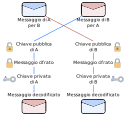
\includegraphics[width=0.5\textwidth]{figures/rsa_disegno}
	\caption{Esempio di corrispondenza elettronica utilizzando un sistema di crittografia asimmetrica.}
\end{figure}

Con questo metodo di cifratura è possibile anche garantire la provenienza di un messaggio. Riprendiamo l'esempio precedente: l'\emph{utente A} questa volta, prima di cifrare il messaggio usando la chiave pubblica dell'\emph{utente B}, lo cifrerà usando la propria chiave privata e solo in un secondo momento lo ri-crittograferà utilizzando la chiave pubblica di \emph{B}. Quando l'\emph{utente B} riceverà il messaggio e lo decifrerà usando la propria chiave inversa, otterrà ancora un messaggio crittografato. Quel dato messaggio necessiterà poi della chiave pubblica dell'\emph{utente A} per essere decifrato, garantendo in questo modo che il messaggio è stato spedito soltanto dall'\emph{utente A}, unico a possedere la chiave privata con la quale era stato crittografato il messaggio.

Più semplicemente, utilizzando questo metodo di cifratura, l'\emph{utente A} può mandare messaggi a tutti, garantendo la provenienza. Infatti, cifrando il messaggio con la propria chiave privata, chiunque sarà in grado di leggere il messaggio, decifrandolo con la sua chiave pubblica, assicurandosi in tal modo che il mittente sia proprio l'\emph{utente A}.































